\section{Real-Robot Setup}
\label{app:real}

\begin{figure*}[t]
\centering
\setlength{\tabcolsep}{2pt}
\begin{tabular}{@{}ccc@{}}
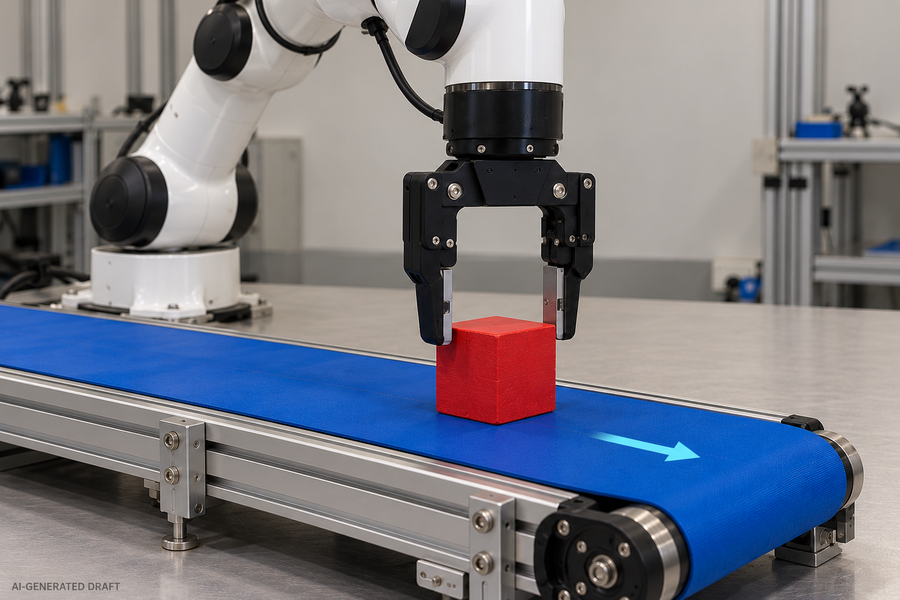
\includegraphics[width=.32\textwidth]{figures/real/01_conveyor_grasping.png} &
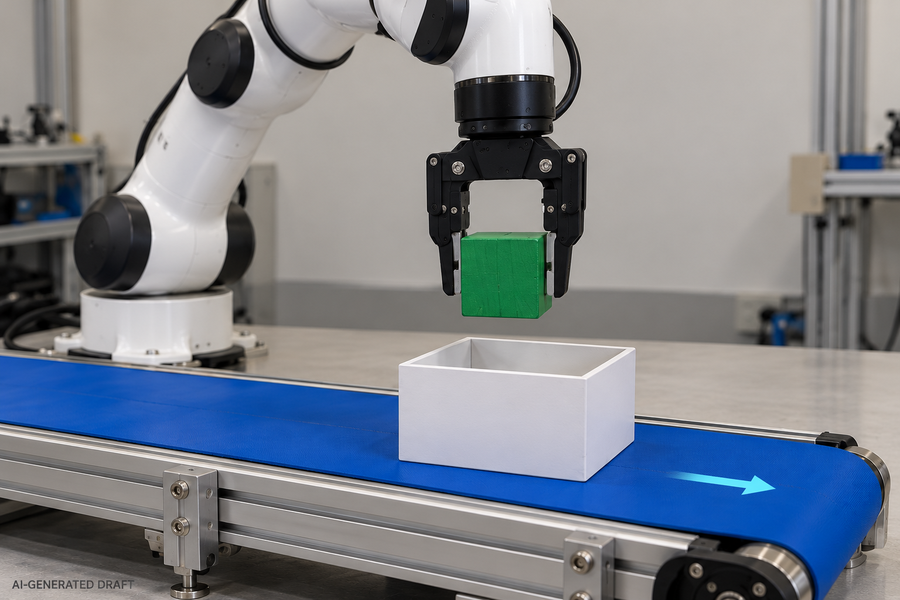
\includegraphics[width=.32\textwidth]{figures/real/02_moving_target_placement.png} &
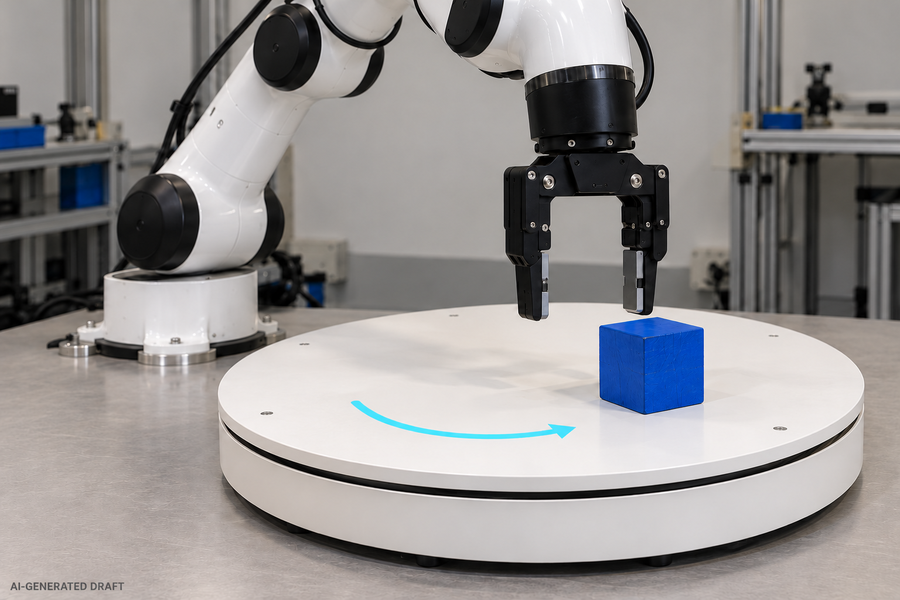
\includegraphics[width=.32\textwidth]{figures/real/03_turntable_grasping.png} \\
\small T1: Conveyor grasping & \small T2: Moving-receptacle placement & \small T3: Turntable grasping \\
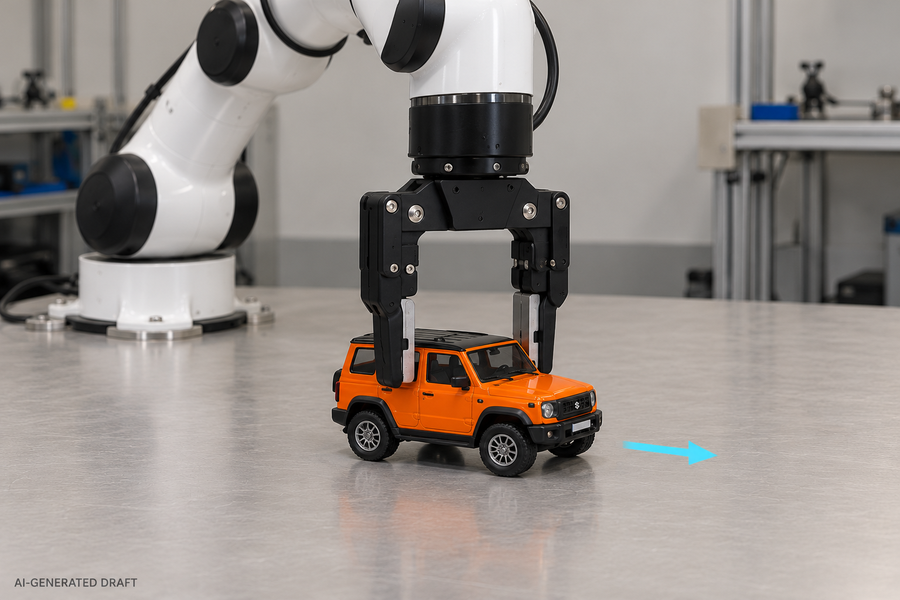
\includegraphics[width=.32\textwidth]{figures/real/04_moving_car_grasping.png} &
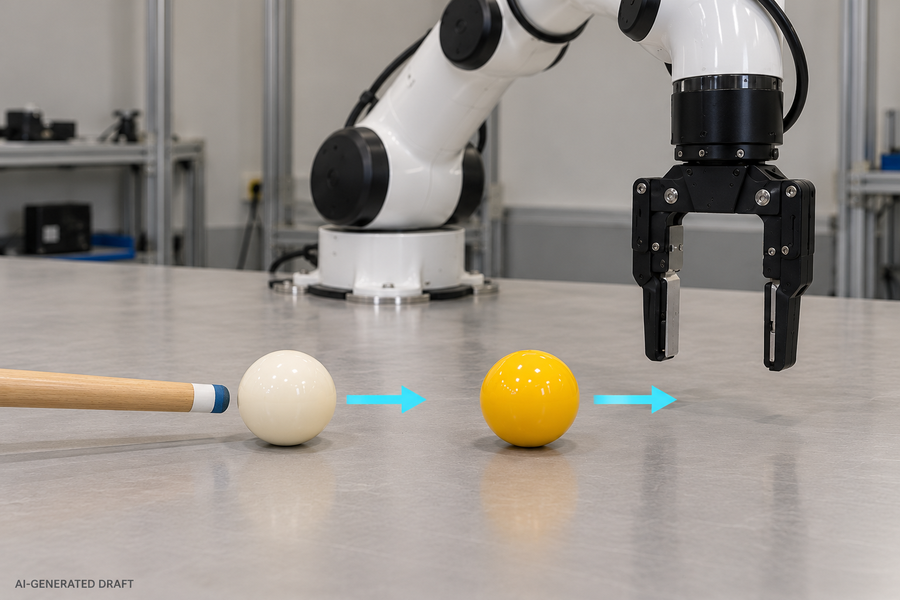
\includegraphics[width=.32\textwidth]{figures/real/05_ball_collision_interception.png} &
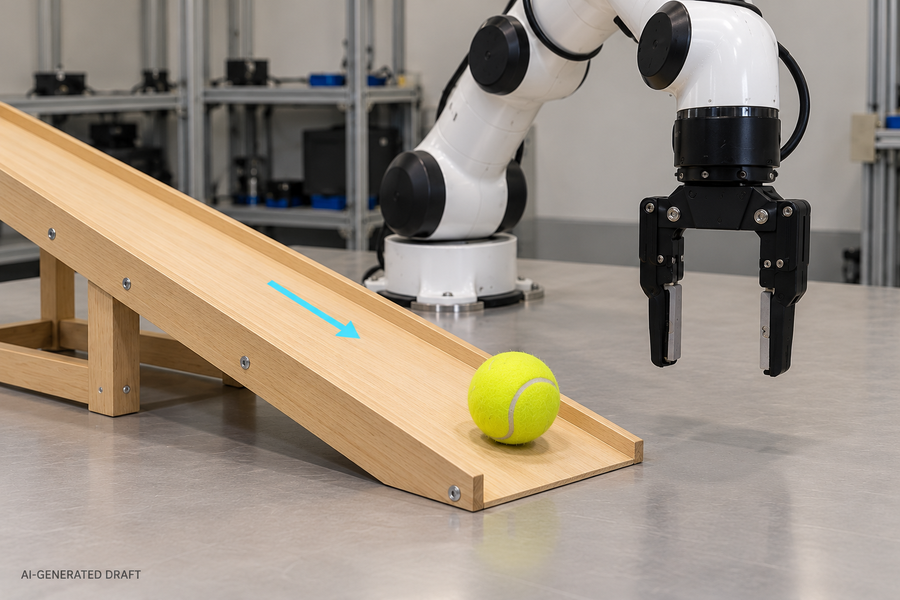
\includegraphics[width=.32\textwidth]{figures/real/06_ramp_interception.png} \\
\small T4: Moving-car grasping & \small T5: Post-collision interception & \small T6: Ramp interception
\end{tabular}
% CONFIRM(real figures): these are AI-generated concept images (visible "AI-GENERATED DRAFT" marks);
% replace them with photographs of the real setup before submission.
\caption{\textbf{Real-robot tasks.} AI-generated concept illustrations, to be
replaced by photographs of the setup; arrows indicate the intended target motion.
T6 shows the rolling variant; the task also includes sliding objects.}
\label{fig:real_setup}
\end{figure*}

\subsection{Platform and Tasks}
\label{app:real_platform}
The robot is \cfgRobot{}, commanded through \fillin{a timestamped Cartesian
interface} at \fillin{control frequency}. The camera records RGB-D at
\fillin{resolution} and \fillin{frame rate}, and we calibrate its extrinsics by
\fillin{procedure} before each session. \ours uses this fixed third-person view;
baselines whose recipes require a wrist view receive \fillin{per-method camera
configuration}. All policies run on one \cfgGPU{}. Table~\ref{tab:real_tasks} defines
the six tasks. T1 and T2 share a belt conveyor, T3 uses a turntable, T4 a remotely
driven toy car, T5 a cue-driven collision between two balls, and T6 a ramp. Touching
or pushing the target without completing the task, a single-finger hold, and an
action after the target has left the workspace count as failures;
\fillin{equipment-invalid trials and safety interventions are repeated or counted as
failures by the following rule}.

\begin{table*}[t]
\centering\footnotesize
\caption{Real-robot task definitions. $N=100$: training demonstrations per task;
20 additional demonstrations per task are reserved for validation.}
\label{tab:real_tasks}
\setlength{\tabcolsep}{3pt}
\begin{tabular}{@{}p{.05\textwidth}p{.37\textwidth}p{.22\textwidth}p{.25\textwidth}@{}}
\toprule
Task & Device, motion, and objects & Operating range; $N$ & Success and failure criteria \\
\midrule
T1 & Conveyor transports a graspable cube. & \fillin{belt speed}; 100 & \fillin{stable grasp and lift; failures} \\
T2 & Conveyor transports an open box; the arm places a cube into it. & \fillin{belt speed}; 100 & \fillin{placement and retention; failures} \\
T3 & Turntable carries a cube around its axis. & \fillin{angular speed, radius}; 100 & \fillin{stable grasp and lift; failures} \\
T4 & Remotely driven toy car moves on the tabletop. & \fillin{speed, path}; 100 & \fillin{car grasp and lift; failures} \\
T5 & A cue-driven ball strikes a second ball; the arm intercepts the second ball after the collision. & \fillin{impact and outgoing speed}; 100 & \fillin{post-impact capture; failures} \\
T6 & A ball rolls or a block slides down a ramp toward the interception region. & \fillin{slope, release, speed}; 100 & \fillin{capture and retention; failures} \\
\bottomrule
\end{tabular}
\end{table*}

\subsection{Pose Tracking}
\label{app:tracker}
Tracking is marker-free. Each object has one fixed reference model with a shared
origin, axes, and scale across all demonstrations and trials. Grounding DINO
\cite{groundingdino} localizes the object named by the task in the first frame, SAM~2.1
\cite{sam2} propagates its mask causally, and \fillin{the tracker, e.g., FoundationPose
\cite{foundationpose}} registers the masked RGB-D observation to the reference.
\fillin{Image resolution, reference acquisition, and loss and recovery thresholds.}
The tracker runs in its own thread. Each estimate carries its capture time,
availability time, and validity, is issued once, and is never revised by later
frames. Training labels for the demonstrations use the same object frame with
multiframe registration. For the ball tasks, the target-state tokens keep the
translation, velocity, and acceleration of the ball center and mask its orientation
and angular motion, and the pose head is supervised on translation only.
Table~\ref{tab:supp_tracker} reports the tracking accuracy.

% Planned results: selected marker-free pipeline; real errors require an independent marker-free reference with stated uncertainty. No tracker ranking or ball rotation experiment.
\begin{table}[t]
\centering\footnotesize
\caption{\tablelang{\textbf{Real-robot pose tracking.} Median/p95 translation (mm) and rotation ($^\circ$) error of the tracker against a marker-free reference, the uncertainty of that reference, and the fraction of lost observations. Ball rotation is not used.}{\textbf{真机位姿跟踪。}跟踪器相对无标记参照的平移（mm）与旋转（$^\circ$）误差的中位数/p95、该参照的不确定度，以及观测丢失比例。球体不使用旋转。}}
\label{tab:supp_tracker}
\setlength{\tabcolsep}{2.8pt}
\begin{tabular}{@{}lcccc@{}}
\toprule
\tablelang{Target}{目标} & mm & $^\circ$ & \tablelang{Ref.\ uncertainty}{参照不确定度} & \tablelang{Lost}{丢失} \\
\midrule
\tablelang{Real rigid object}{真机刚体} & \resultplaceholder[{0.0/0.0}] & \resultplaceholder[{0.0/0.0}] & \resultplaceholder & \resultplaceholder \\
\tablelang{Real ball}{真机球体} & \resultplaceholder[{0.0/0.0}] & -- & \resultplaceholder & \resultplaceholder \\
\bottomrule
\end{tabular}
\end{table}


\subsection{Trials}
\label{app:real_trials}
We compare \ours, $\pi_{0.5}$, DynamicWAM, and Diffusion Policy
\cite{diffusionpolicy}, with 20 trials per task and method. All methods use the same
pre-generated trial keys, which fix the object instance, the initial pose, and the
motion parameters, sampled by \fillin{sampling protocol}. Trials run in
\fillin{randomized method order}, so that drift of the apparatus does not align with
the methods. An operator resets the scene. A trial starts at the first usable
observation, the robot may move at any time, and a trial ends at success, failure,
or a timeout of \fillin{X}\,s. Demonstrations, development trials, and test trials
come from separate sessions. \ours is fine-tuned per task from the DROID base
(Appendix~\ref{app:posttraining}), and the baselines are trained or fine-tuned on the
same demonstrations with \fillin{per-method initialization and training settings}.
Table~\ref{tab:supp_real_ci} reports successes per task, 95\% binomial intervals for
the pooled rates, and paired differences from a bootstrap over trial keys.

% Planned results: six-task real-robot study (App. D.3); per-task counts, baseline set, and numeric results to be filled (see docs/writing/v4_t5_real_report.md).
\begin{table*}[t]
\centering\footnotesize
\caption{\tablelang{\textbf{Real-robot successes} per task (successes/trials, \fillin{n} trials per task; tasks in Table~\ref{tab:real_tasks}). All: pooled success rate (\%) with its 95\% binomial interval. $\Delta$: paired difference from \ours (points) with a bootstrap interval over trial keys. $e_t$: median contact-time error (ms) on trials that make contact.}{\textbf{真机成功次数}，按任务分列（成功次数/试验数，每个任务 \fillin{n} 次；任务定义见表~\ref{tab:real_tasks}）。All：合并成功率（\%）及 95\% 二项区间。$\Delta$：相对 \ours 的配对差值（百分点）及按试验键自助法得到的区间。$e_t$：发生接触的试验中接触时刻误差的中位数（ms）。}}
\label{tab:supp_real_ci}
\setlength{\tabcolsep}{3pt}
\begin{tabular}{@{}lccccccccc@{}}
\toprule
\tablelang{Method}{方法} & T1 & T2 & T3 & T4 & T5 & T6 & All & $\Delta$ & $e_t$ \\
\midrule
\fillin{$\pi_{0.5}$} & \resultplaceholder[s/n] & \resultplaceholder[s/n] & \resultplaceholder[s/n] & \resultplaceholder[s/n] & \resultplaceholder[s/n] & \resultplaceholder[s/n] & \resultplaceholder[00.0 {[00, 00]}] & \resultplaceholder[{$-$00.0 [00, 00]}] & \resultplaceholder \\
\fillin{DynamicWAM} & \resultplaceholder[s/n] & \resultplaceholder[s/n] & \resultplaceholder[s/n] & \resultplaceholder[s/n] & \resultplaceholder[s/n] & \resultplaceholder[s/n] & \resultplaceholder[00.0 {[00, 00]}] & \resultplaceholder[{$-$00.0 [00, 00]}] & \resultplaceholder \\
\tablelang{\ours, no DROID base}{\ours，无 DROID 基座} & \resultplaceholder[s/n] & \resultplaceholder[s/n] & \resultplaceholder[s/n] & \resultplaceholder[s/n] & \resultplaceholder[s/n] & \resultplaceholder[s/n] & \resultplaceholder[00.0 {[00, 00]}] & \resultplaceholder[{$-$00.0 [00, 00]}] & \resultplaceholder \\
\ours & \resultplaceholder[s/n] & \resultplaceholder[s/n] & \resultplaceholder[s/n] & \resultplaceholder[s/n] & \resultplaceholder[s/n] & \resultplaceholder[s/n] & \resultplaceholder[00.0 {[00, 00]}] & -- & \resultplaceholder \\
\bottomrule
\end{tabular}
\end{table*}

